\section{Zuständigkeiten}
\label{section_zustaendigkeiten}
In diesem Kapitel wird auf die Zuständigkeiten im Bezug auf Informationsbereitstellung an der Hochschule Emden/Leer eingegangen. Es wird dargestellt, welche Bereiche bereits zentral an der Informationsbereitstellung beteiligt sind und wo bereits Synergien vorliegen. Ebenso wird auf die Besonderheiten einzelner Fachbereiche, zentrale Einrichtungen und das Präsidium detaillierter eingegangen. 

\begin{figure}[h!]
	\centering
	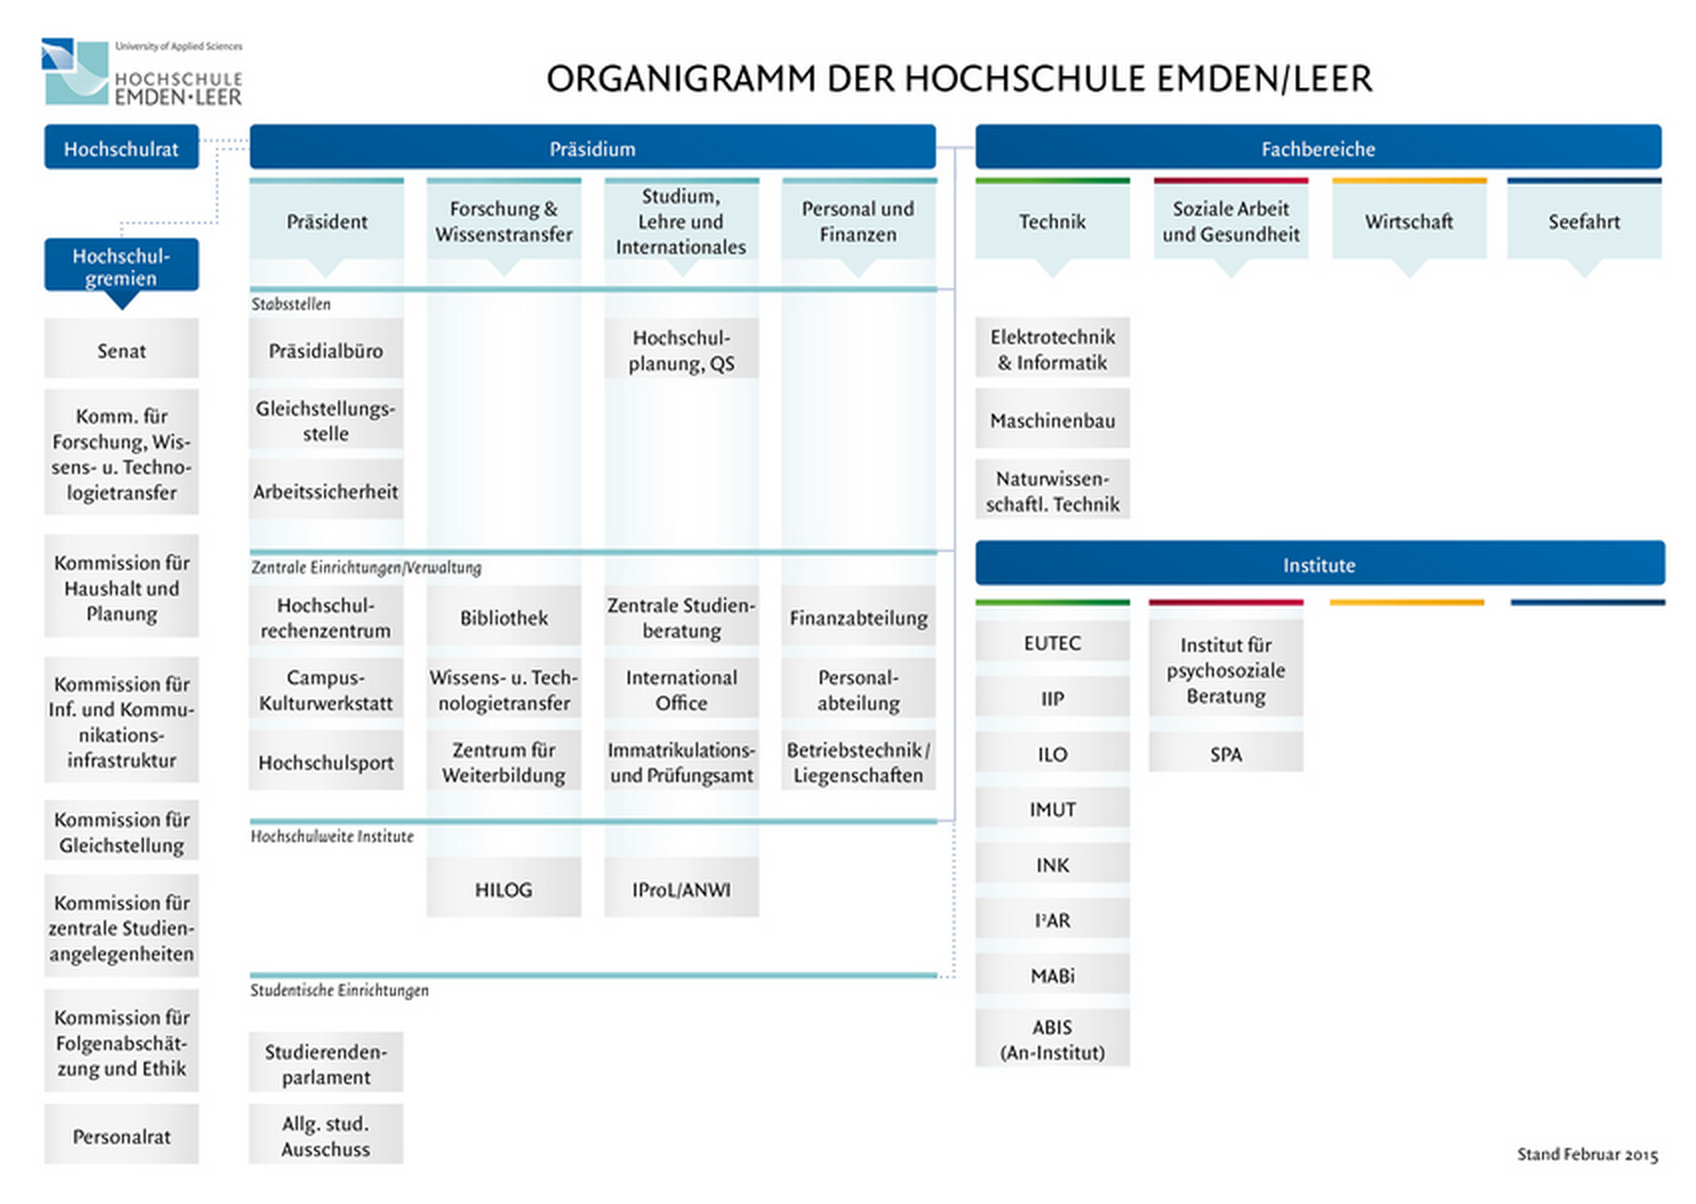
\includegraphics[width=14cm]{kapitel/gruppe2/bilder/organigramm_HS}
	\caption{Organigramm der Hochschule Emden/Leer}
	\label{fig_organigramm_HS}
\end{figure}

\missingfigure{Schaubild über zentral genutzte Systeme unabhängig von Kooperation}

\subsection{Fachbereiche}
Die einzelnen Fachbereiche sind unter anderem durch die Mitgliedschaft in Arbeitsgruppen in den Informationsbeschaffungsprozess involviert (siehe Kapitel \ref{subsection_arbeitsgruppen_informationsaustausch}). 

Alle Fachbereiche verfügen über die Berechtigung relevante Informationen in dem Infosys darzustellen. Infosys ist eine zentrale Plattform, welche online auf der Webseite der Hochschule Emden/Leer öffentlich von jedem eingesehen werden kann oder vor Ort  in den Eingangsbereichen der jeweiligen Fachbereiche über Dashboards. Es werden, nach Fachbereich sortiert, die wichtigsten Neuigkeiten als Newsticker dargestellt und der Zugriff auf alle Vorlesungspläne der Fachbereiche ist gegeben um so zügig auf organisatorische Inhalte zugreifen zu können.

\missingfigure{Screenshot Info Sys}

In den nachfolgenden Kapiteln wird nur auf die Besonderheiten der einzelnen Fachbereiche eingegangen.

\subsubsection{Seefahrt}
Bei dem Fachbereich Seefahrt handelt es sich um einen relativ kleinen Fachbereich. Seefahrt ist  nur an dem Standort Leer vertreten. Dieser Fachbereich verwendet kein zentrales System zur Vorlesung und Raumplanung, sondern eine Eigenentwicklung.

\subsubsection{Technik}
Eine Besonderheit dieses Fachbereiches ist, dass für den Laborbetrieb ein Rechennetz neben dem zentralen Rechennetz der Hochschule Emden/Leer betrieben wird. Da unter anderem der Bereich „IT-Sicherheit“ ein wichtiger Aspekt in dem Studiengang Informatik ist, kommt es zu besonderen Konstellationen im Bereich der Forschung. Dieser Bereich verwaltet sein Netz selbst und ist somit autark vom allgemeinen Hochschulrechennetz.

\subsubsection{Wirtschaft}
\subsubsection{Soziale Arbeit und Gesundheit}

\subsection{Präsidium}
Das Präsidium insbesondere mit dem Bereich zentrale Verwaltung ist durch die Mitgliedschaft in Arbeitsgruppen in den Informationsbeschaffungsprozess involviert. Eine besondere Stelle, im Bezug auf die Repräsentation von Informationen besonders das Erscheinungsbild nach außen (siehe Kapitel \ref{section_kooperations_situation}), stellt eine Stabsstelle von dem Präsidium da. Das Präsidialbüro ist unter anderem für den Bereich Hochschulmarketing zuständig.

\subsection{Zentrale Verwaltung}
(\ldots)
\subsubsection{Studentenverwaltung}
\subsubsection{Mitarbeiterverwaltung}
\subsubsection{Rechenzentrum}
Das Hochschulrechenzentrum der Hochschule Emden/Leer ist stark in die Administration und Pflege der bestehenden Systeme zur Informationsbereitstellung involviert. Neben der Administration von bestehenden Systemen obliegt dem Hochschulrechenzentrum ebenfalls der Endkundensupport.

\subsection{Arbeitsgruppen zum Informationsaustausch und zur Informationsbereitstellung}
\label{subsection_arbeitsgruppen_informationsaustausch}
Die Zuständigkeiten an der Hochschule, in Bezug auf Informationssammlung, Beschaffung und Aufbereitung von Informationen, ist bereits durch Arbeitsgruppen in wichtigen Bereichen geregelt. Durch das Interview mit dem Leiter des Hochschulrechenzentrums der Hochschule Emden/Leer konnte ein Einblick in die bestehenden Gremien geschaffen werden. Derzeit existieren drei Arbeitsgruppen, welche für die Informationsverteilung in den jeweiligen Bereichen relevant sind:

\begin{itemize}
	\item Zahlen, Daten und Fakten (ZDF)
	\item WEB
	\item Moodle
\end{itemize}

\subsubsection{Zahlen, Daten und Fakten (ZDF)}
ZDF setzt sich zusammen aus den Verwaltungsabteilungen Finanzen, Personal, Presse und Rechenzentrum. Dieses Gremium ist zuständig für die Aufbereitung und zur Verfügung Stellung von Kennzahlen wie zum Beispiel aktuelle Kennzahlen zu eingeschriebenen Studierenden pro Studiengang.  ZDF ist für einen Unterbereich der offiziellen Webseite der Hochschule Emden/Leer zuständig. Die Kennzahlen und Zahlen werden gruppenbasiert erstellt. Es werden grobe Kennzahlen erzeugt, welche öffentlich zugänglich sind und detailliertere Zahlen für die Mitarbeiter, mit welchen sie arbeiten können. Dekane erhalten speziellere Zahlenwerte.

\subsubsection{WEB}
Es existiert eine Arbeitsgruppe, welche für die Gestaltung und den Inhalt der öffentlichen Webseite der Hochschule Emden/Leer verantwortlich ist. In dieser Arbeitsgruppe sind aus jedem Fachbereich Repräsentanten mit einbezogen. Die Leitung des Web-Teams obliegt dem Präsidialbüro.\footnote{\url{http://www.hs-emden-leer.de/fileadmin/user_upload/Einrichtungen/Praesidialbuero/Organigramm_Praesidialbuero_Juli2013_01.pdf}}

\subsubsection{Moodle}
In der Arbeitsgruppe „Moodle“ sind sowohl Repräsentanten aus jedem Fachbereich involviert sowie auch Repräsentanten aus der Verwaltungsebene. Da das Moodle E-learning System mittlerweile als ein zentrales Moodle für alle Bereiche eingeführt wurde, haben die Mitglieder aus den Fachbereichen unter anderem das Recht Kurse im Moodle freischalten zu können. 
